\iffalse
\documentclass[10pt,a4paper]{report}
\usepackage[latin1]{inputenc}
\usepackage{amsmath}
\usepackage{amsfonts}
\usepackage{amssymb}
\usepackage{graphicx}
\usepackage{hyperref}
\usepackage{multicol}
\usepackage[margin=0.5in]{geometry}
\usepackage{tikz}
\usepackage[document]{ragged2e}
\usepackage{romannum}
\usetikzlibrary{arrows,shapes.gates.logic.US,shapes.gates.logic.IEC,calc}
\usepackage{titlesec}
\titlespacing{\subsection}{1pt}{\parskip}{3pt}
\titlespacing{\subsubsection}{0pt}{\parskip}{-\parskip}
\titlespacing{\paragraph}{0pt}{\parskip}{\parskip}
\newcommand{\myvec}[1]{\ensuremath{\begin{pmatrix}#1\end{pmatrix}}}
\let\vec\mathbf

\newcommand{\mydet}[1]{\ensuremath{\begin{vmatrix}#1\end{vmatrix}}}
\providecommand{\brak}[1]{\ensuremath{\left(#1\right)}}
\providecommand{\lbrak}[1]{\ensuremath{\left(#1\right.}}
\providecommand{\rbrak}[1]{\ensuremath{\left.#1\right)}}
\providecommand{\sbrak}[1]{\ensuremath{{}\left[#1\right]}}

\begin{document}

\begin{multicols}{2}
\raggedright {
\includegraphics[scale=0.06]{IITH logo.jpg}} \vspace{3mm}\\ \raggedleft Name:SHAIK KHAJA MASTAN AHMED\vspace{2mm}\\ 
\raggedleft Roll No.: FWC22052\vspace{2mm}\\ 
\raggedleft 19pa1a04e9@vishnu.edu.in \vspace{2mm}\\ 
\raggedleft Oct 2022 \vspace{5mm}\\
\end{multicols}

\centering \Large \textbf{OPTIMIZATION ASSIGNMENT} \normalsize \vspace{10mm}

%\begin{multicols}{2}

\section{Problem:}  
\fi
Find the maximum area of an isosceles triangle inscribed in the ellipse $\frac{x^2}{a^2} + \frac{y^2}{b^2} = 1$ with its vertex at one end of the major axis.
\\
\solution
\iffalse
\section{Solution: }

\raggedright \textbf{Input Parameters :}\\ \vspace{2mm}
\centering Ellipse Equation : $\frac{x^2}{a^2} + \frac{y^2}{b^2} = 1$. \\ \vspace{1mm}
Vertex is at one end of the major axis.
\vspace{3mm}

\raggedright \textbf{To Find :}\\ \vspace{2mm}
\begin{enumerate}
\item Comparing the given equation with the equation of the ellipse and finding it's parameters and the major axis.
\item Finding the vertices of the triangle lies on the ellipse and required equation for area of the triangle.
\item Evaluating the Area of triangle.
\item Finding the maximum area of the triangle inscribed in the ellipse.
\end{enumerate}

\raggedright \textbf{Step - 1 :}\\ \vspace{2mm}
Ellipse Equation : $\frac{x^2}{a^2} + \frac{y^2}{b^2} = 1$. \\ \vspace{1mm}
Let us assume the lengths of major and minor axis be 5,3 respectively.
\begin{align*}
i.e., a=5 \\
b=3
\end{align*}
The equation of the ellipse is given as :
\begin{align}
\vec{x}^{\top}\vec{V}\vec{x}+f=0
\end{align}
The given equation can be expressed with \\parameters
\begin{align}
	\vec{V} &= \myvec{b^2 & 0\\0 & a^2}, f = -a^2b^2.
	\end{align}
Here the major axis is 
\begin{align}
\myvec{0&1}\vec{x}=0
\end{align}

\raggedright \textbf{Step - 2 :}\\ \vspace{2mm}
The vertex is at one end of the major axis be (a,0),
Assuming the other two points on the ellipse, so isosceles triangle can be formed\\ \vspace{1mm}
The vertices be :
\begin{align}
\vec{x_1}=\myvec{a\\0} , \vec{x_2}=\myvec{x_1\\x_2}, \vec{x_3}=\myvec{y_1\\y_2}
\end{align}
The height and the side of the triangle are perpendicular to each other.\\
The line vector of height is major axis of the ellipse. 
i.e.,
\begin{align*}
\myvec{0&1} \vec{x}=0
\end{align*}
\begin{align}
\myvec{0&1}\myvec{x_1-y_1\\x_2-y_2}=0
\end{align}
using dot product we get,
\begin{align}
\therefore x_1=y_1
\end{align}
Since the given triangel is isosceles,
\begin{align}
\|\vec{x_1}-\vec{x_2}\|=\|\vec{x_1}-\vec{x_3}\|
\end{align}
\begin{align*}
\implies \sqrt{|\vec{x_1}|^2+|\vec{x_2}|^2-2\vec{x_1.x_2^T}}=\sqrt{|\vec{x_1}|^2+|\vec{x_3}|^2-2\vec{x_1.x_3^T}}
\end{align*}
\begin{align}
\implies \vec{x_2}=\pm \vec{x_3}
\end{align}
\begin{align*}
\implies \myvec{x_1\\x_2}=\pm \myvec{y_1\\y_2}
\end{align*}
\begin{align*}
\implies \myvec{x_1\\x_2}=\myvec{x_1\\ \pm y_2}
\end{align*}
\begin{align}
\therefore y_2 = - x_2
\end{align}
\centering Here we should consider $-y_2$. \\Because, if we consider $+y_2$ then the points will be same. so, it cannot form a triangle.\\ \vspace{3mm}

The area of the triangle can be obtained by
\begin{align}
A=\frac{1}{2} |(\vec{x_1}- \vec{x_2}) \times (\vec{x_1} - \vec{x_3)}|
\end{align}
\begin{align}
\implies \frac{1}{2} \Big| \myvec{a-x_1 & a-x_1\\x_2 & -x_2} \Big|
\end{align}
upon simplification we get,
\begin{align}
\vec{A}=\vec{ax_2-x_1x_2}
\end{align}

\raggedright \textbf{Step - 3 :}\\ \vspace{2mm}
The vertices of triangle lies on the ellipse in (1)
\begin{align*}
\myvec{x&y}\myvec{b^2&0\\0&a^2}\myvec{x\\y}=a^2b^2
\end{align*}
\begin{align}
y=\frac{b}{a}\sqrt{a^2-x^2}
\end{align}

\centering By substituting (13) in $x_2$ at (12). \\We get Area of triangle
\begin{align}
\implies A=b\sqrt{a^2-x^2}+\frac{b}{a}x\sqrt{a^2-x^2}
\end{align}
The above equation i.e.,(14) is the area of the isosceles triangle in one variable.\\
Upon derivating the above equation(14), we get:
\begin{align}
\nabla A = \frac{ba^2-2bx^2-abx}{a\sqrt{a^2-x^2}}
\end{align}

\raggedright \textbf{Step - 4 :}\\ \vspace{2mm}
The maximum area of the triangle will be calculated by finding the local maxima of the function.\\
using gradient ascent method we can find its maxima,
\begin{align}
x_{n+1} &= x_n + \alpha \nabla V \\
\implies x_{n+1} &= x_n + \alpha \brak{\frac{ba^2-2bx^2-abx}{a\sqrt{a^2-x^2}}}
\end{align}

\section{Plot :}
\begin{center}
  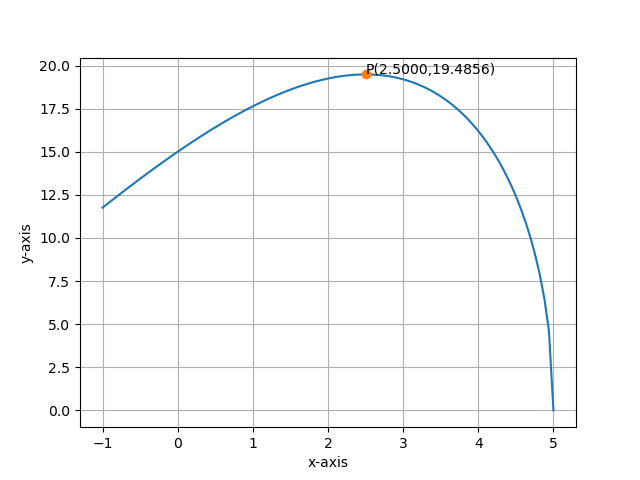
\includegraphics[scale=0.55]{optimization.png}
  Figure-1
  \end{center}



Taking $x_0=1,\alpha=0.001$ and precision = 0.00000001, values obtained using python are:
    
    \begin{align}
        \boxed{\text{Maxima} = 19.485571582762454}\\
        \boxed{\text{Maxima Point} = 2.499952069714825}
    \end{align}
    
\raggedright \textbf{Code Link :}\\ \vspace{2mm}
The below link realises the code of the above construction.\\
\begin{center}
\fbox{\parbox{8.5cm}{\url{https://github.com/19pa1a04e9/FWC-IITH/tree/main/Assignment-1/OPTIMIZATION/codes/optimization.py}}}
\end{center}

\section{Termux Commands :}
\centering bash rncom.sh ..... Using Shell commands.

%\end{multicols}
\end{document}
\fi
